\documentclass[10pt,a4paper]{article}

\usepackage{a4wide}
\setlength{\parskip}{0.5ex plus0.1ex minus0.1ex}
\setlength{\parindent}{0em}

\usepackage[round,longnamesfirst]{natbib}
\usepackage{hyperref}

%%% for tabulars
\usepackage{rotating}
\usepackage{multirow}

\newcommand{\strong}[1]{{\normalfont\fontseries{b}\selectfont #1}}
\newcommand{\class}[1]{\mbox{\textsf{#1}}}
\newcommand{\func}[1]{\mbox{\texttt{#1()}}}
\newcommand{\code}[1]{\mbox{\texttt{#1}}}
\newcommand{\pkg}[1]{\strong{#1}}
\newcommand{\samp}[1]{`\mbox{\texttt{#1}}'}
\newcommand{\proglang}[1]{\textsf{#1}}
\newcommand{\set}[1]{\mathcal{#1}}

\usepackage{Sweave}
%% \VignetteIndexEntry{Introduction to arules}


\begin{document}
%% ------------------------------------------------------------------
%% ------------------------------------------------------------------
\title{Introduction to \pkg{arules} -- Mining 
    Association Rules and Frequent Item Sets}
\author{Michael Hahsler and Bettina Gr{\"u}n and Kurt Hornik}
\maketitle
\sloppy
%% ------------------------------------------------------------------
%% ------------------------------------------------------------------
\begin{abstract}
  Mining frequent itemsets and association rules is a popular and well
  researched approach for discovering interesting relationships between
  variables in large databases.  The \proglang{R} package \pkg{arules}
  presented in this paper provides a basic infrastructure for creating
  and manipulating input data sets and for analyzing the resulting
  itemsets and rules.  The package also includes interfaces to two fast
  mining algorithms, the popular \proglang{C} implementations of Apriori
  and Eclat by Christian Borgelt.  These algorithms can be used to mine
  frequent itemsets, maximal frequent itemsets, closed frequent itemsets
  and association rules.
\end{abstract}

%% ------------------------------------------------------------------
%% ------------------------------------------------------------------

\section{Introduction}

Mining frequent itemsets and association rules is a popular and well
researched method for discovering interesting relations between
variables in large databases. \cite{arules:Piatetsky-Shapiro:1991}
describes analyzing and presenting strong rules discovered in databases
using different measures of interest.  Based on the concept of strong
rules, \cite{arules:Agrawal+Imielinski+Swami:1993} introduced the
problem of mining association rules from transaction data as follows:

Let $I=\{i_1, i_2,\ldots,i_n\}$ be a set of $n$ binary attributes called
\emph{items}.  Let $\set{D} = \{t_1, t_2, \ldots, t_m\}$ be a set of
transactions called the \emph{database}.  Each transaction
in~$\set{D}$ has an unique transaction ID and
contains a subset of the items in~$I$.
A \emph{rule} is defined as an implication of the form $X \Rightarrow Y$
where $X, Y \subseteq I$ and $X \cap Y = \emptyset$.  The sets of items
(for short \emph{itemsets}) $X$ and $Y$ are called \emph{antecedent}
(left-hand-side or LHS) and \emph{consequent} (right-hand-side or RHS)
of the rule.

\begin{figure}
\centering
  \begin{tabular}{|c|l|}
  \hline
  {\bf transaction} ID & {\bf items}\\  
  
  \hline
  1 & milk, bread \\
  2 & bread, butter \\
  3 & beer \\
  4 & milk, bread, butter \\
  5 & bread, butter \\
  \hline
\end{tabular}
\caption{An example supermarket database with five transactions.\label{table:supermarket}}
\end{figure}

To illustrate the concepts, we use a small example from the supermarket
domain.  The set of items is $I= \{\mathrm{milk, bread, butter, beer}\}$
and a small database containing the items is shown in
Figure~\ref{table:supermarket}.  An example rule for the supermarket
could be $\{\mathrm{milk, bread}\} \Rightarrow \{\mathrm{butter}\}$
meaning that if milk and bread is bought, customers also buy butter.

To select interesting rules from the set of all possible rules,
constraints on various measures of significance and interest can be
used.  The best-known constraints are minimum thresholds on support and
confidence.  The \emph{support}~$\mathrm{supp}(X)$ of an itemset~$X$ is
defined as the proportion of transactions in the data set which contain
the itemset.  In the example database in Figure~\ref{table:supermarket},
the itemset $\{\mathrm{milk, bread}\}$ has a support of $2/5=0.4$ since
it occurs in 40\% of all transactions (2 out of 5 transactions).

Finding frequent
itemsets can be seen as a simplification of the unsupervised learning
problem called ``mode finding'' or ``bump
hunting''~\citep{arules:Hastie+Tibshirani+Friedman:2001}.  For these
problems each item is seen as a variable.  The goal is to find prototype
values so that the probability density evaluated at these values is
sufficiently large.  However, for practical applications with a large
number of variables, probability estimation will be unreliable and
computationally too expensive.  This is why in practice frequent
itemsets are used instead of probability estimation.

The \emph{confidence} of a rule is defined $\mathrm{conf}(X\Rightarrow
Y) = \mathrm{supp}(X \cup Y) / \mathrm{supp}(X)$.  For example, the rule
$\{\mathrm{milk, bread}\} \Rightarrow \{\mathrm{butter}\}$ has a
confidence of $0.2/0.4=0.5$ in the database in
Figure~\ref{table:supermarket}, which means that for 50\% of the
transactions containing milk and bread the rule is correct.
Confidence can be interpreted as an estimate of the probability
$P(Y|X)$, the probability of finding the RHS of the rule in transactions
under the condition that these transactions also contain the LHS
\citep[see e.g.,][]{arules:Hipp+Guentzer+Nakhaeizadeh:2000}.

Association rules are required to satisfy both a minimum support and a
minimum confidence constraint at the same time.  At medium to low
support values, often a great number of frequent itemsets are found in a
database.  However, since the definition of support enforces that all
subsets of a frequent itemset have to be also frequent, it is sufficient
to only mine all \emph{maximal frequent itemsets}, defined as frequent
itemsets which are not proper subsets of any other frequent
itemset~\citep{arules:Zaki+Parthasarathy+Ogihara+Li:1997}.  Another
approach to reduce the number of mined itemsets is to only mine
\emph{frequent closed itemsets.}  An itemset is closed if no proper
superset of the itemset is contained in each transaction in which the
itemset is contained~\citep{arules:Pasquier+Bastide+Taouil+Lakhal:1999,
  arules:Zaki:2004}.  Frequent closed itemsets are a superset of the
maximal frequent itemsets.  Their advantage over maximal frequent
itemsets is that in addition to yielding all frequent itemsets, they
also preserve the support information for all frequent itemsets which
can be important for computing additional interest measures after the
mining process is finished (e.g., confidence for rules generated from
the found itemsets, or
\emph{all-confidence}~\citep{arules:Omiecinski:2003}).


A practical solution to the problem of finding too many association
rules satisfying the support and confidence constraints is to further
filter or rank found rules using additional interest measures.  A
popular measure for this purpose is
\emph{lift}~\citep{arules:Brin+Motwani+Ullman+Tsur:1997}.  The lift of a
rule is defined as $\mathrm{lift}(X \Rightarrow Y) = \mathrm{supp}(X
\cup Y) / (\mathrm{supp}(X) \mathrm{supp}(Y))$, and can be interpreted
as the deviation of the support of the whole rule from the support
expected under independence given the supports of the LHS and the RHS.
Greater lift values indicate stronger associations.


In the last decade, research on algorithms to solve the frequent itemset
problem has been abundant.  \cite{arules:Goethals+Zaki:2004} compare the
currently fastest algorithms.  Among these algorithms are the
implementations of the Apriori and Eclat algorithms by
\cite{arules:Borgelt:2003} interfaced in the \pkg{arules} environment.
The two algorithms use very different mining strategies.  Apriori,
developed by \cite{arules:Agrawal+Srikant:1994}, is a level-wise,
breadth-first algorithm which counts transactions.  In contrast, Eclat
\citep{arules:Zaki+Parthasarathy+Ogihara+Li:1997} employs equivalence
classes, depth-first search and set intersection instead of counting.
The algorithms can be used to mine frequent itemsets, maximal frequent
itemsets and closed frequent itemsets.  The implementation of Apriori
can additionally be used to generate association rules.

This paper presents \pkg{arules}, an extension package for
\proglang{R}~\citep{arules:R:2005} which provides the infrastructure
needed to create and manipulate input data sets for the mining
algorithms and for analyzing the resulting itemsets and rules.  Since it
is common to work with large sets of rules and itemsets, the package
uses sparse matrix representations to minimize memory usage.  The
infrastructure provided by the package was also created to explicitly
facilitate extensibility, both for interfacing new algorithms and for
adding new types of interest measures and associations.

The rest of the paper is organized as follows: In the next section, we
give an overview of the data structures implemented in the
package~\pkg{arules}.
%In Sections~\ref{sec:transactions} and \ref{sec:associations} 
In Section~\ref{sec:overview} we introduce the functionality of the
classes to handle transaction data and associations.  In
Section~\ref{sec:interfaces} we describe the way mining algorithms are
interfaced in \pkg{arules} using the available interfaces to Apriori and
Eclat as examples.  In Section~\ref{sec:auxiliary} we present some
auxiliary methods for support counting, rule induction and sampling
available in \pkg{arules}.  We provide several examples in
%Sections~\ref{sec:example-screen} to \ref{sec:example-allconf}.
Section~\ref{sec:examples}.  The first two examples show typical
\proglang{R} sessions for preparing, analyzing and manipulating a
transaction data set, and for mining association rules.  The third
example demonstrates how \pkg{arules} can be extended to integrate a new
interest measure.  Finally, the fourth example shows how to use sampling
in order to speed up the mining process.  We conclude with a summary of
the features and strengths of the package~\pkg{arules} as a
computational environment for mining association rules and frequent
itemsets.

A previous version of this manuscript was published in the \emph{Journal
  of Statistical Software} \citep{arules:Hahsler+Gruen+Hornik:2005b}.


%% ------------------------------------------------------------------
%% ------------------------------------------------------------------
\section{Data structure overview\label{sec:overview}}

To enable the user to represent and work with input and output data of
association rule mining algorithms in \proglang{R}, a well-designed
structure is necessary which can deal in an efficient way with large
amounts of sparse binary data.  The \proglang{S4} class structure
implemented in the package \pkg{arules} is presented in
Figure~\ref{fig:arules-classes}.

\begin{figure}[tp]
\centering
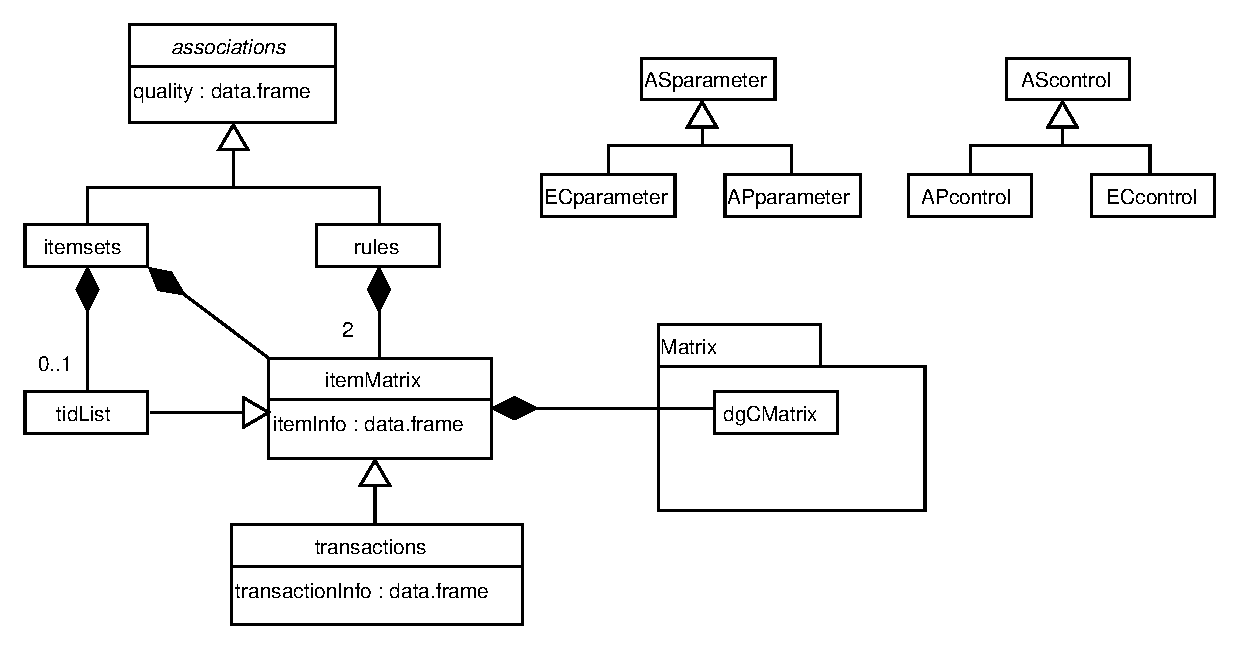
\includegraphics[width=12cm]{arules-classes}
\caption{UML class diagram \citep[see][]{misc:Fowler:2004} of the \pkg{arules}
package.\label{fig:arules-classes}}
\end{figure}

For input data the classes \class{transactions} and \class{tidLists}
(transaction ID lists, an alternative way to represent transaction data)
are provided.  The output of the mining algorithms comprises the classes
\class{itemsets} and \class{rules} representing sets of itemsets or
rules, respectively.  Both classes directly extend a common virtual
class called \class{associations} which provides a common interface.  In
this structure it is easy to add a new type of associations by adding a
new class that extends \class{associations}.

Items in \class{associations} and \class{transactions} are implemented
by the \class{itemMatrix} class which provides a facade for the sparse
matrix implementation \class{ngCMatrix} from the \proglang{R} package
\pkg{Matrix}~\citep{arules:Bates+Maechler:2005}.

To control the behavior of the mining algorithms, the two classes
\class{ASparameter} and \class{AScontrol} are used.  Since each
algorithm can use additional algorithm-specific parameters, we
implemented for each interfaced algorithm its own set of control
classes.  We used the prefix \samp{AP} for Apriori and \samp{EC} for
Eclat.  In this way, it is easy to extend the control classes when
interfacing a new algorithm.


\subsection{Representing collections of itemsets\label{sec:setrepresentation}}

From the definition of the association rule mining problem we see that
transaction databases and sets of associations have in common that 
they contain sets of items (itemsets) together with additional information.
For example, a transaction in the database 
% $\set{D}$ 
contains a transaction ID and an itemset.
A rule in a set of mined association rules 
% $\set{R}$
contains two itemsets, one for the LHS and one for the RHS, 
and additional quality information, e.g., values for various interest measures.



\begin{figure}[tp]
\centering
%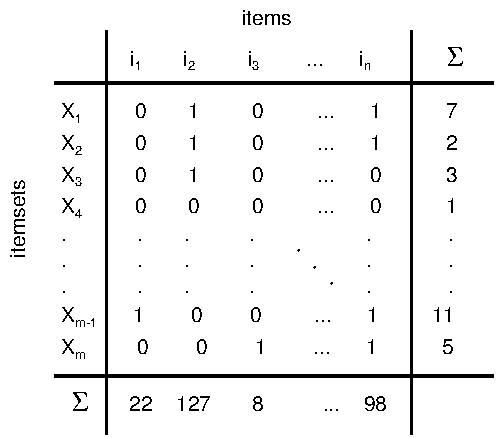
\includegraphics[width=5cm]{itemsetMatrix}

\renewcommand{\arraystretch}{1.1}
\setlength{\tabcolsep}{2mm}
\begin{tabular}{cl|cccc}
%\begin{tabular}{cl|ccccc}
%& & \multicolumn{5}{c}{items}\\
& & \multicolumn{4}{c}{items}\\

%%& & $i_1$ & $i_2$ & $i_3$ &  . . . & $i_n$ \\
& & $i_1$ & $i_2$ & $i_3$ &  $i_4$ \\
& & milk & bread & butter  & beer \\
%\hline
\cline{2-6}
%\multirow{9}{1.5ex}{ \begin{sideways} itemsets \end{sideways} }
%\multirow{8}{1.5ex}{ \begin{sideways} itemsets \end{sideways} }
\multirow{4}{*}{\begin{sideways} itemsets \end{sideways}}

%& $X_1$ 		& 0 & 1 & 0 & . . . & 1 \\
%& $X_2$ 	  	& 0 & 1 & 0 & . . . & 1 \\
%& $X_3$ 		& 0 & 1 & 0 & . . . & 0 \\
%& $X_4$ 		& 0 & 0 & 1 & . . . & 0 \\
%& \phantom{-}.&.&.&.&\hspace{-7mm}.&.\\
%& \phantom{-}.&.&.&.&.&.\\
%& \phantom{-}.&.&.&.&\hspace{7mm}.&.\\
%& $X_{m-1}$ 		& 1 & 0 & 0 & . . . & 1 \\
%& $X_m$ 		& 0 & 0 & 1 & . . . & 1 \\

& $X_1$ 		& 1 & 1 & 0 &  0 \\
& $X_2$ 	  	& 0 & 1 & 0 &  1 \\
& $X_3$ 		& 1 & 1 & 1 &  0 \\
& $X_4$ 		& 0 & 0 & 1 &  0 \\
%& \phantom{-}.&.&.&.&.\\
%& \phantom{-}.&.&.&.&.\\
%& \phantom{-}.&.&.&.&.\\
%& $X_{m-1}$ 		& 1 & 0 & 0 & 1 \\
%& $X_m$ 		& 0 & 1 & 1 & 0 \\
\end{tabular}
\caption{Example of a collection of itemsets represented as a 
    binary incidence matrix.\label{fig:itemsetMatrix}}
\end{figure}

Collections of itemsets used for transaction databases and sets of
associations can be represented as binary incidence matrices with
columns corresponding to the items and rows corresponding to the
itemsets.  The matrix entries represent the presence (1) or absence (0)
of an item in a particular itemset.  An example of a binary incidence
matrix containing itemsets for the example database in
Figure~\ref{table:supermarket} on Page~\pageref{table:supermarket} is
shown in Figure~\ref{fig:itemsetMatrix}.  Note that we need to store
collections of itemsets with possibly duplicated elements (identical
rows), i.e, itemsets containing exactly the same items. This is
necessary, since a transaction database can contain different
transactions with the same items. Such a database is still a set of
transactions since each transaction also contains a unique
transaction~ID.

Since a typical frequent itemset or a typical transaction (e.g., a
supermarket transaction) only contains a small number of items compared
to the total number of available items, the binary incidence matrix will
in general be very sparse with many items and a very large number of
rows.  A natural representation for such data is a sparse matrix format.
For our implementation we chose the \class{ngCMatrix} class defined in
package~\pkg{Matrix}.  The \class{ngCMatrix} is a compressed, sparse, logical,
column-oriented matrix which contains the indices of the \code{TRUE} rows and
the pointers to the initial indices of elements in each column of the matrix.
Despite the column orientation of the \class{ngCMatrix}, it is more convenient
to work with incidence matrices which are row-oriented.  This makes the most
important manipulation, selecting a subset of transactions from a data set for
mining, more comfortable and efficient.  Therefore, we implemented the class
\class{itemMatrix} providing a row-oriented facade to the \class{ngCMatrix}
which stores a transposed incidence matrix\footnote{Note that the developers of
package~\pkg{Matrix} contains some support for a sparse row-oriented format,
but the available functionality currently is rather minimal.  Once all required
functionality is implemented, \pkg{arules} will switch the internal
representation to sparse row-oriented logical matrices.}.  
In sparse representation the following
information needs to be stored for the collection of itemsets in
Figure~\ref{fig:itemsetMatrix}: A vector of indices of the non-zero
elements (row-wise starting with the first row) $1, 2, 2, 4, 1, 2, 3, 3$
and the pointers $1, 3, 5, 8$ where each row starts in the index vector.
The first two pointers indicate that the first row starts with element
one in the index vector and ends with element 2 (since with element 3
already the next row starts).  The first two elements of the index
vector represent the items in the first row which are $i_1$ and $i_2$ or
milk and bread, respectively.  The two vectors are stored in the
\class{ngCMatrix}. Note that indices for the \class{ngCMatrix} start
with zero rather than with one and thus actually the vectors $0, 1, 1,
3, 0, 3, 3$ and $0, 3, 4, 7$ are stored.  However, the data structure of
the \class{ngCMatrix} class is not intended to be directly accessed by
the end user of \pkg{arules}. The interfaces of \class{itemMatrix} can
be used without knowledge of how the internal representation of the data
works.  However, if necessary, the \class{ngCMatrix} can be directly
accessed by developers to add functionality to \pkg{arules} (e.g., to
develop new types of associations or interest measures or to efficiently
compute a distance matrix between itemsets for clustering).  In this
case, the \class{ngCMatrix} should be accessed using the coercion
mechanism from \class{itemMatrix} to \class{ngCMatrix} via \func{as}.

In addition to the sparse matrix, \class{itemMatrix} stores item labels
(e.g., names of the items) and handles the necessary mapping between the
item label and the corresponding column number in the incidence matrix.
Optionally, \class{itemMatrix} can also store additional information on
items.  For example, the category hierarchy in a supermarket setting can
be stored which enables the analyst to select only transactions (or as
we later see also rules and itemsets) which contain items from a certain
category (e.g., all dairy products).

For \class{itemMatrix}, basic matrix operations including \func{dim} and
subset selection (\code{[}) are available.  The first element of
\func{dim} and \code{[} corresponds to itemsets or transactions (rows),
the second element to items (columns).  For example, on a transaction
data set in variable \code{x} the subset selection \samp{x[1:10, 16:20]}
selects a matrix containing the first 10 transactions and items 16 to
20.

Since \class{itemMatrix} is used to represent sets 
or collections of itemsets additional functionality is provided.
\func{length} can be used to get the number of itemsets in an
\class{itemMatrix}.
Technically, \func{length} returns the number of rows in the matrix
which is equal to the first element returned by \func{dim}.
%\pkg{arules} also provides set operations including \func{union},
%\func{intersect} and \func{setequal}.
Identical itemsets can be found with \func{duplicated}, and duplications
can be removed with \func{unique}.  \func{match} can be used to find
matching elements in two collections of itemsets.

With \func{c}, several \class{itemMatrix} objects can be combined by
successively appending the rows of the objects, i.e., creating a
collection of itemsets which contains the itemsets from all
\class{itemMatrix} objects.  This operation is only possible if the
\class{itemMatrix} objects employed are ``compatible,'' i.e., if the
matrices have the same number of columns and the items are in the same
order.  If two objects contain the same items (item labels), but the
order in the matrix is different or one object is missing some items,
\func{recode} can be used to make them compatible by reordering and
inserting columns.


To get the actual number of items in the itemsets stored in the
\class{itemMatrix}, \func{size} is used.  It returns a vector with the
number of items (ones) for each element in the set (row sum in the
matrix).  Obtaining the sizes from the sparse representations is a very
efficient operation, since it can be calculated directly from the vector
of column pointers in the \class{ngCMatrix}.  For a purchase incidence
matrix, \func{size} will produce a vector as long as the number of
transactions in the matrix with each element of the vector containing
the number of items in the corresponding transaction.  This information
can be used, e.g., to select or filter unusually long or short
transactions.

\func{itemFrequency} calculates the frequency for each item in an
\class{itemMatrix}. Conceptually, the item frequencies are the column sums of
the binary matrix. Technically, column sums can be implemented for sparse
representation efficiently by just tabulating the vector of row numbers of the
non-zero elements in the \class{ngCMatrix}.  Item frequencies can be used for
many purposes.  For example, they are needed to compute interest measures.
\func{itemFrequency} is also used by \func{itemFrequencyPlot} to produce a bar
plot of item count frequencies or support.  Such a plot gives a quick overview
of a set of itemsets and shows which are the most important items in terms of
occurrence frequency.


Coercion from and to \class{matrix} and \class{list} primitives is
provided where names and dimnames are used as item labels.  For the
coercion from \class{itemMatrix} to \class{list} there are two
possibilities.  The usual coercion via \func{as} results in a list of
vectors of character strings, each containing the item labels of the
items in the corresponding row of the \class{itemMatrix}.  The actual
conversion is done by \func{LIST} with its default behavior (argument
\code{decode} set to \code{TRUE}).  If in turn \func{LIST} is called
with the argument \code{decode} set to \code{FALSE}, the result is a
list of integer vectors with column numbers for items instead of the
item labels. For many computations it is useful to work with such a list
and later use the item column numbers to go back to the original
\class{itemMatrix} for, e.g., subsetting columns.  For subsequently
decoding column numbers to item labels, \func{decode} is also available.

Finally, \func{image} can be used to produce a level plot of an
\class{itemMatrix} which is useful for quick visual inspection.  For
transaction data sets (e.g., point-of-sale data) such a plot can be very
helpful for checking whether the data set contains structural changes (e.g.,
items were not offered or out-of-stock during part of the observation
period) or to find abnormal transactions (e.g., transactions which
contain almost all items may point to recording problems).  Spotting
such problems in the data can be very helpful for data preparation.



%% ------------------------------------------------------------------
%% ------------------------------------------------------------------

\subsection{Transaction data\label{sec:transactions}}

The main application of association rules is for market basket analysis
where large transaction data sets are mined.  In this setting each
transaction contains the items which were purchased at one visit to a
retail store \citep[see e.g.,][]{arules:Berry+Linoff:1997}.
Transaction data are normally recorded by point-of-sale
scanners and often consists of tuples of the form:

\begin{displaymath}
<\emph{transaction ID}, \emph{item ID}, \ldots >
\end{displaymath}

All tuples with the same transaction ID form a single transaction which
contains all the items given by the item IDs in the tuples.  Additional
information denoted by the ellipsis dots might be available.  For
example, a customer ID might be provided via a loyalty program in a
supermarket.  Further information on transactions (e.g., time,
location), on the items (e.g., category, price), or on the customers
(socio-demographic variables such as age, gender, etc.) might also be
available.

\begin{figure}[tp]
\centering
%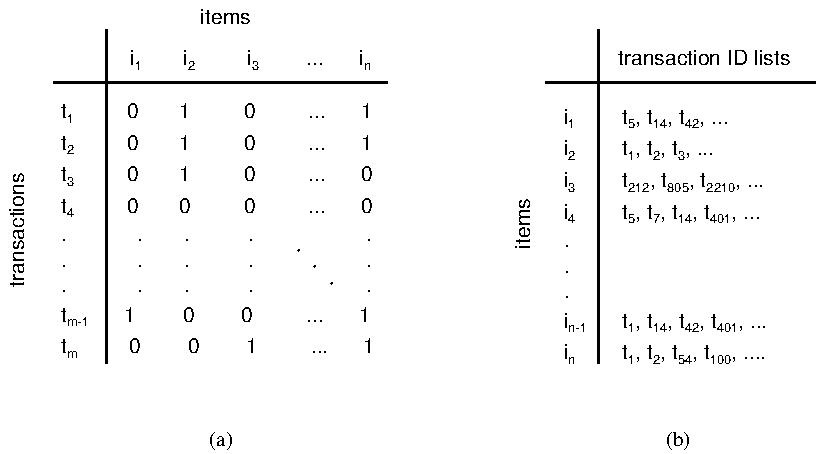
\includegraphics[width=12cm]{transactionMatrix}

\begin{minipage}[b]{.4\linewidth}
\renewcommand{\arraystretch}{1.1}
\setlength{\tabcolsep}{2mm}
%
\begin{center}
\begin{tabular}{cl|cccc}
& & \multicolumn{4}{c}{items}\\

& & milk & bread & butter & beer \\
%\hline
\cline{2-6}
\multirow{5}{*}{\begin{sideways} transactions \end{sideways}}

& 1 		& 1 & 1 & 0 & 0 \\
& 2 	  	& 0 & 1 & 1 & 0 \\
& 3 		& 0 & 0 & 0 & 1 \\
& 4 		& 1 & 1 & 1 & 0 \\
& 5 		& 0 & 1 & 1 & 0 \\
\end{tabular}

\vspace{1cm}
(a)
\end{center}
\end{minipage}
%
\hspace{.1\linewidth}
%
\begin{minipage}[b]{.4\linewidth}
\renewcommand{\arraystretch}{1.1}
\setlength{\tabcolsep}{2mm}
%
\begin{center}
\begin{tabular}{cl|l}
& & \multicolumn{1}{c}{transaction ID lists}\\

%\hline
\cline{2-3}
\multirow{4}{*}{\begin{sideways} items \end{sideways}}

& milk  		& 1, 4 \\
& bread  		& 1, 2, 4, 5 \\
& butter 		& 2, 4 \\
& beer  		& 3 \\
\end{tabular}

\vspace{1.5cm}
(b)
\end{center}
\end{minipage}

\caption{Example of a set of transactions represented in 
    (a) horizontal layout and in 
    (b) vertical layout.\label{fig:transactionMatrix}}
\end{figure}

For mining, the transaction data is first transformed into a binary
purchase incidence matrix with columns corresponding to the different
items and rows corresponding to transactions.  The matrix entries
represent the presence (1) or absence (0) of an item in a particular
transaction.  This format is often called the \emph{horizontal} database
layout~\citep{arules:Zaki:2000}.  Alternatively, transaction data can be
represented in a \emph{vertical} database layout in the form of
\emph{transaction ID lists}~\citep{arules:Zaki:2000}.  In this format
for each item a list of IDs of the transactions the item is contained in
is stored.  In Figure~\ref{fig:transactionMatrix} the example database
in Figure~\ref{table:supermarket} on Page~\pageref{table:supermarket} is
depicted in horizontal and vertical layouts.  Depending on the
algorithm, one of the layouts is used for mining.  In \pkg{arules} both
layouts are implemented as the classes~\class{transactions} and
\class{tidLists}.  Similar to \class{transactions},
class~\class{tidLists} also uses a sparse representation to store its
lists efficiently.  Objects of classes~\class{transactions} and
\class{tidLists} can be directly converted into each other by coercion.

The class \class{transactions} directly extends \class{itemMatrix} and
inherits its basic functionality (e.g., subset selection, getting
itemset sizes, plotting item frequencies).  In addition,
\class{transactions} has a slot to store further information for each
transaction in form of a \class{data.frame}.  The slot can hold
arbitrary named vectors with length equal to the number of stored
transactions.  In \pkg{arules} the slot is currently used to store
transaction IDs, however, it can also be used to store user IDs, revenue
or profit, or other information on each transaction.  With this
information subsets of transactions (e.g., only transactions of a
certain user or exceeding a specified profit level) can be selected.

Objects of class \class{transactions} can be easily created by coercion
from \class{matrix} or \class{list}.  If names or dimnames are available
in these data structures, they are used as item labels or transaction
IDs, accordingly.  To import data from a file, the
\func{read.transactions} function is provided.  This function reads
files structured as shown in Figure~\ref{fig:transactionMatrix} and also
the very common format with one line per transaction and the items
separated by a predefined character.  Finally, \func{inspect} can be
used to inspect transactions (e.g., ``interesting'' transactions
obtained with subset selection).

Another important application of mining association rules has been
proposed by \cite{arules:Piatetsky-Shapiro:1991} and
\cite{arules:Srikant+Agrawal:1996} for discovering interesting
relationships between the values of categorical and quantitative
(metric) attributes.  For mining associations rules, non-binary
attributes have to be mapped to binary attributes. The straightforward
mapping method is to transform the metric attributes into $k$ ordinal
attributes by building categories (e.g., an attribute income might be
transformed into a ordinal attribute with the three categories: ``low'',
``medium'' and ``high'').  Then, in a second step, each categorical
attribute with $k$ categories is represented by $k$ binary dummy
attributes which correspond to the items used for mining.  An example
application using questionnaire data can be found in
\cite{arules:Hastie+Tibshirani+Friedman:2001} in the chapter
about association rule mining.

The typical representation for data with categorical and quantitative
attributes in \proglang{R} is a \class{data.frame}.  First, a domain
expert has to create useful categories for all metric attributes.  This
task is supported in \proglang{R} by functions such as \func{cut}.  The
second step, the generation of binary dummy items, is automated in
package \pkg{arules} by coercing from \class{data.frame} to
\class{transactions}.  In this process, the original attribute names and
categories are preserved as additional item information and can be used
to select itemsets or rules which contain items referring to a certain
original attributes.
By default it is assumed that missing values do not carry information and thus
all of the corresponding dummy items are set to zero.  
If the fact
that the value of a specific attribute is missing provides information 
(e.g., a respondent in an interview refuses to answer a specific question), 
the domain expert can create for the attribute a category for missing values 
which then will be included in the transactions as its own dummy item.

The resulting \class{transactions} object can be
mined and analyzed the same way as market basket data, see the example
in Section~\ref{sec:example-screen}.


%% ------------------------------------------------------------------
%% ------------------------------------------------------------------
\subsection{Associations: itemsets and sets of rules\label{sec:associations}}

The result of mining transaction data in \pkg{arules} are
\class{associations.}  Conceptually, associations are sets of objects
describing the relationship between some items (e.g., as an itemset or a
rule) which have assigned values for different measures of quality.
Such measures can be measures of significance (e.g., support), or
measures of interest (e.g., confidence, lift), or other measures (e.g.,
revenue covered by the association).

All types of association have a common functionality in \pkg{arules} comprising
the following methods:
\begin{itemize}
 \item \func{summary} to give a short overview of the set and
  \func{inspect} to display individual associations,
 \item \func{length} for getting the number of elements in the set,
 \item \func{items} for getting for each association a set of items
  involved in the association (e.g., the union of the items in the LHS
  and the RHS for each rule),
 \item sorting the set using the values of different quality measures
  (\func{SORT}),
 \item subset extraction (\code{[} and \func{subset}),
 \item set operations (\func{union}, \func{intersect} and
  \func{setequal}), and
 \item matching elements from two sets (\func{match}),
% \item handling of duplicated elements for a collection
%     of associations (\func{duplicated} and \func{unique}).
\item \func{WRITE} for writing associations to disk in human readable form.
  To save and load associations in compact form, 
  use \func{save} and \func{load} from the
  \pkg{base} package. Package \pkg{pmml}~\citep{arules:Williams:2008} 
  includes functionality to
  save associations in PMML (Predictive Modelling Markup Language).
\end{itemize}

The associations currently implemented in package~\pkg{arules} are sets
of itemsets (e.g., used for frequent itemsets of their closed or maximal
subset) and sets of rules (e.g., association rules).  Both classes,
\class{itemsets} and \class{rules}, directly extend the virtual class
\class{associations} and provide the functionality described above.

Class \class{itemsets} contains one \class{itemMatrix} object to store
the items as a binary matrix where each row in the matrix represents an
itemset. In addition, it may contain transaction ID lists as an object
of class \class{tidLists}.  Note that when representing transactions,
\class{tidLists} store for each item a transaction list, but here store
for each itemset a list of transaction IDs in which the itemset appears.
Such lists are currently only returned by \func{eclat}.

Class \class{rules} consists of two \class{itemMatrix} objects
representing the left-hand-side (LHS) and the right-hand-side (RHS) of
the rules, respectively.

The items in the associations and the quality measures can be accessed
and manipulated in a safe way using accessor and replace methods for
\code{items}, \code{lhs}, \code{rhs}, and \code{quality}.  In addition
the association classes have built-in validity checking which ensures
that all elements have compatible dimensions.

It is simple to add new quality measures to existing associations.
Since the \code{quality} slot holds a \class{data.frame}, additional
columns with new quality measures can be added. These new measures can
then be used to sort or select associations using \func{SORT} or
\func{subset}.  Adding a new type of associations to \pkg{arules} is
straightforward as well. To do so, a developer has to create a new class
extending the virtual \class{associations} class and implement the
common functionality described above.

%% ------------------------------------------------------------------
%% ------------------------------------------------------------------

\section{Mining algorithm interfaces\label{sec:interfaces}}

In package \pkg{arules} we interface free reference implementations of
Apriori and Eclat by Christian Borgelt
\citep{arules:Borgelt+Kruse:2002,arules:Borgelt:2003}.  The code is
called directly from \proglang{R} by the functions \func{apriori} and
\func{eclat} and the data objects are directly passed from \proglang{R} to
the \proglang{C} code and back without writing to external files.
The implementations can mine frequent itemsets,
and closed and maximal frequent itemsets. 
In addition, \func{apriori} can also mine association rules.  

The data given to the \func{apriori} and \func{eclat} functions have to
be \class{transactions} or something which can be coerced to
\class{transactions} (e.g., \class{matrix} or \class{list}).  The
algorithm parameters are divided into two groups represented by the
arguments \code{parameter} and \code{control}.  The mining parameters
(\code{parameter}) change the characteristics of the mined itemsets or
rules (e.g., the minimum support) and the control parameters
(\code{control}) influence the performance of the algorithm (e.g.,
enable or disable initial sorting of the items with respect to their
frequency).  These arguments have to be instances of the classes
\class{APparameter} and \class{APcontrol} for the function
\func{apriori} or \class{ECparameter} and \class{ECcontrol} for the
function \func{eclat}, respectively.  Alternatively, data which can be
coerced to these classes (e.g., \code{NULL} which will give the default
values or a named list with names equal to slot names to change the
default values) can be passed.  In these classes, each slot specifies a
different parameter and the values.  The default values are equal to the
defaults of the stand-alone \proglang{C} programs
\citep{arules:Borgelt:2004} except that the standard definition of the
support of a rule \citep{arules:Agrawal+Imielinski+Swami:1993} is
employed for the specified minimum support required (Borgelt defines the
support of a rule as the support of its antecedent).

For \func{apriori} the appearance feature implemented by Christian
Borgelt can also be used.  With argument \code{appearance} of function
\func{apriori} one can specify which items have to or must not appear in
itemsets or rules.  For more information on this feature we refer to the
Apriori manual~\citep{arules:Borgelt:2004}.

The output of the functions \func{apriori} and \func{eclat} is an object
of a class extending \class{associations} which contains the sets of mined
associations and can be further analyzed using the functionality provided for
these classes.


There exist many different algorithms which 
which use an
incidence matrix or transaction ID list representation as input and
solve the frequent and
closed frequent itemset problems.  Each algorithm has specific strengths
which can be important for very large databases.  Such algorithms, e.g.
kDCI, LCM, FP-Growth or Patricia, are discussed
in~\cite{arules:Goethals+Zaki:2003}.  The source code of most algorithms
is available on the internet and, if a special algorithm is needed, 
interfacing the
algorithms for \pkg{arules} is straightforward.
The necessary steps are:

\begin{enumerate}
 \item Adding interface code to the algorithm, preferably by directly
  calling into the native implementation language (rather than using
  files for communication), and an \proglang{R} function calling this
  interface.
 \item Implementing extensions for \class{ASparameter} and
  \class{AScontrol}.
\end{enumerate}



\section{Auxiliary functions \label{sec:auxiliary}}

In \pkg{arules} several helpful functions are implemented for
support counting, rule induction, sampling, etc.
In the following we will discuss some of these functions.

\subsection{Counting support for itemsets\label{sec:counting}}

Normally, itemset support is counted during mining the database with a
given minimum support constraint.  During this process all frequent
itemsets plus some infrequent candidate itemsets are counted (or support
is determined by other means).  Especially for databases with many items
and for low minimum support values, this procedure can be extremely time
consuming since in the worst case, the number of frequent itemsets grows
exponentially in the number of items.

If only the support information for a single or a few itemsets is needed,
we might not want to mine the database for all frequent itemsets. 
We also do not know in advance how high (or low) to set the minimum support to
still get the support information for the itemsets in question.
For this problem, \pkg{arules} contains \func{support}
which determines the support for a set of given sets of items
(as an \class{itemMatrix}).

For counting, we use a prefix tree~\citep{arules:Knuth:1997} to organize the
counters. The used prefix tree is similar to the itemset tree described
by~\cite{arules:Borgelt+Kruse:2002}. However, we do not generate the tree
level-wise, but we first generate a prefix tree which only contains the nodes
necessary to hold the counters for all itemsets which need to be counted.
Using the nodes in this tree only, we count the itemsets for each
transaction recursively. After counting, the support for each itemset is
contained in the node with the prefix equal to the itemset. The exact
procedure is described in~\cite{arules:Hahsler+Buchta+Hornik:2007}.

In addition to determining the support of a few itemsets without mining all
frequent itemsets, \func{support} is also useful for finding 
the support of infrequent itemsets with a support so low that mining
is infeasible due to combinatorial explosion.


\subsection{Rule induction\label{sec:induction}}

For convenience we introduce $\set{X} = \{X_1, X_2, \ldots, X_l\}$ for
sets of itemsets with length $l$.  Analogously, we write $\set{R}$ for
sets of rules.  A part of the association rule mining problem is the
generation (or induction) of a set of rules~$\set{R}$ from a set of
frequent itemsets~$\set{X}$.  The implementation of the Apriori
algorithm used in \pkg{arules} already contains a rule induction engine
and by default returns the set of association rules of the form $X
\Rightarrow Y$ which satisfy given minimum support and minimum
confidence.  Following the definition of
\cite{arules:Agrawal+Imielinski+Swami:1993} $Y$ is restricted to single
items.

In some cases it is necessary to separate mining itemsets and generating
rules from itemsets. For example, only rules stemming from a subset of
all frequent itemsets might be of interest to the user.  The Apriori
implementation efficiently generates rules by reusing the data
structures built during mining the frequent itemsets.  However, if
Apriori is used to return only itemsets or Eclat or some other algorithm
is used to mine itemsets, the data structure needed for rule induction
is no longer available for computing rule confidence.

If rules need to be induced from an arbitrary set of itemsets, support
values required to calculate confidence are typically missing.  For
example, if all available information is an itemset containing five
items and we want to induce rules, we need the support of the itemset
(which we might know), but also the support of all subsets of length
four. The missing support information has to be counted from the
database. Finally, to induce rules efficiently for a given set of
itemsets, we also have to store support values in a suitable data
structure which allows fast look-ups for calculating rule confidence.

Function~\func{ruleInduction} provided in \pkg{arules} 
uses a prefix tree to induce rules for a given
confidence from an arbitrary set of itemsets $\set{X}$ in the following
way:

\begin{enumerate}
    \item Count  the support values for each itemset $X \in \set{X}$ and the
        subsets $\{X \setminus \{x\}: x \in X\}$ needed for rule generation
        in a single pass over the database
        and store them in a suitable data structure.
    \item Populate set $\set{R}$ by selectively generating only rules for the
        itemsets in $\set{X}$ using the support information
        from the data structure created in step 1.
\end{enumerate}


Efficient support counting is done as described in Section~\ref{sec:counting}
above. After counting, all necessary support counts are contained in the prefix
tree. We can retrieve the needed support values and generating the rules is
straight forward. The exact procedure is described
in~\cite{arules:Hahsler+Buchta+Hornik:2007}.


\subsection{Sampling from transactions\label{sec:sample}}

Taking samples from large databases for mining is a powerful technique
which is especially useful if the original database does not fit into
main memory, but the sample does.  However, even if the database fits
into main memory, sampling can provide an enormous speed-up for mining
at the cost of only little degradation of accuracy.

\cite{arules:Mannila+Toivonen+Verkamo:1994}
proposed sampling with replacement for association rule mining
and quantify the estimation error due to sampling.
Using Chernov bounds on the binomial distribution (the number of
transactions which contains a given itemset in a sample),
the authors argue that in theory even relatively small samples 
should provide good estimates for support.

\cite{arules:Zaki+Parthasarathy+Li+Ogihara:1997} built upon the
theoretic work by \cite{arules:Mannila+Toivonen+Verkamo:1994} and show
that for an itemset $X$ with support $\tau = \mathrm{supp}(X)$ and for
an acceptable relative error of support $\epsilon$ (an accuracy of $1 -
\epsilon$) at a given confidence level $1-c$, the needed sample size~$n$
can be computed by

\begin{equation}
n = \frac{-2\mathrm{ln}(c)}{\tau\epsilon^2}.
\label{equ:samplesize}
\end{equation}

Depending on its support, for each itemset a different sample size is
appropriate.  As a heuristic, the authors suggest to use the user
specified minimum support threshold for $\tau$.  This means that for
itemsets close to minimum support, the given error and confidence level
hold while for more frequent itemsets the error rate will be less.
However, with this heuristic the error rate for itemsets below minimum
support can exceed $\epsilon$ at the given confidence level and thus
some infrequent itemsets might appear as frequent ones in the sample.

\cite{arules:Zaki+Parthasarathy+Li+Ogihara:1997} also evaluated sampling
in practice on several data sets and conclude that sampling not only
speeds mining up considerably, but also the errors are considerably
smaller than those given by the Chernov bounds and thus samples with
size smaller than obtained by Equation~\ref{equ:samplesize} are often
sufficient.

Another way to obtain the required sample size 
for association rule mining is progressive 
sampling~\citep{arules:Parthasarathy:2002}.
This approach starts with a small sample and uses progressively larger 
samples until model accuracy does not improve significantly anymore. 
\cite{arules:Parthasarathy:2002} defines a proxy for 
model accuracy improvement by using a similarity measure between two
sets of associations. The idea is that 
since larger samples will produce more accurate results, the
similarity between two sets of associations of two consecutive samples
is low if accuracy improvements are high and increases with
decreasing accuracy improvements.
Thus increasing sample size can be stopped if the similarity
between consecutive samples reaches a ``plateau.'' 

\cite{arules:Toivonen:1996} presents an application of sampling to reduce
the needed I/O overhead for very large databases which do not fit into 
main memory.
The idea is to use a random sample from the data base to mine
frequent itemsets at a support threshold below the set minimum support.
The support of these itemsets is then counted in the whole database 
and the infrequent itemsets are discarded. 
If the support threshold to mine the sample is picked low enough, 
almost all frequent itemsets and their support will be found
in one pass over the large database.

In \pkg{arules} sampling is implemented by \func{sample}
which provides all capabilities of the standard sampling function 
in \proglang{R}
(e.g., sampling with or without replacement and probability weights).


%\subsection{Random transactions}
%The function \func{random.transactions} can be used to create a random 
%transaction data set of given size and with given marginal probabilities 
%for the items.
%Each transaction is the result of one independent Bernoulli trial for each 
%item resulting in a data set 
%which only contains noise and no structure.
%Such data sets can be
%used to test how well interest measures are able to suppress noise.

%% ------------------------------------------------------------------
%% ------------------------------------------------------------------


\subsection{Sub-, super-, maximal and closed itemsets}
For some calculations it is necessary to find all sub- or supersets 
for a specific itemset
in a set of itemsets. This functionality is implemented as 
\func{is.subset} and \func{is.superset}. 
For example, \code{is.subset(x, y, proper = TRUE)}, finds all
proper subsets of the itemsets in \code{x} in the set~\code{y}. 
The result is a logical matrix with \code{length(x)} 
rows and \code{length(y)} columns.  Each logical row vector represents 
which elements in \code{y} are subsets of the corresponding element in 
\code{x}. If \code{y} is omitted, the sub- or superset structure within the
set \code{x} is returned.

Similar methods, \func{is.maximal} and \func{is.closed}, can be used to find all
\emph{maximal itemsets} or \emph{closed itemsets} in a set.  An itemset is
maximal in a set if no proper superset of the itemset is contained in the
set~\citep{arules:Zaki+Parthasarathy+Ogihara+Li:1997}.  An itemset is closed,
if it is its own closure (i.e., for an items no superset with the same support
exits)~\citep{arules:Pasquier+Bastide+Taouil+Lakhal:1999}.


Note that these methods can be extremely slow and have high memory 
usage if the set contains many itemsets. 

\subsection{Additional measures of interestingness}
\pkg{arules} provides 
\func{interestMeasure}
which can be used to calculate
a broad variety of interest measures for itemsets and rules. 
All measures are calculated
using the quality information available from the
sets of itemsets or rules (i.e., support, confidence, lift) and,
if necessary, missing information is obtained from the
transactions used to mine the associations.

For example, available measures for itemsets are:
\begin{itemize}
\item All-confidence~\citep{arules:Omiecinski:2003}
\item Cross-support ratio~\citep{arules:Xiong+Tan+Kumar:2003}
\end{itemize}

For rules the following measures are implemented:
\begin{itemize}
\item Chi square measure~\citep{arules:Liu+Hsu+Ma:1999}
\item Conviction~\citep{arules:Brin+Motwani+Ullman+Tsur:1997} 
\item Hyper-lift and hyper-confidence~\citep{arules:Hahsler+Hornik:2007} 
\item Leverage~\citep{arules:Piatetsky-Shapiro:1991} 
\item Improvement~\citep{arules:Bayardo+Agrawal+Gunopulos:2000} 
\item Several measures from \cite{arules:Tan+Kumar+Srivastava2004} 
  (e.g., cosine, Gini index, $\phi$-coefficient, odds ratio)
\end{itemize}

\subsection{Distance based clustering transactions and associations}

To allow for distance based clustering~\citep{arules:Gupta+Strehl+Ghosh:1999},
\pkg{arules} provides \func{dissimilarity} which can be used to calculate
dissimilarities and cross-dissimilarities between transactions or associations
(i.e., itemsets and rules). Currently, the following standard measures for
binary data are available: Jaccard coefficient, simple matching coefficient and
dice coefficient. Additionally, dissimilarity between transactions can be
calculated based on affinities between
items~\citep{arules:Aggarwal+Procopiuc+Yu:2002}.

The result of \func{dissimilarity} is either a \code{dist} object, which can be
directly used by most clustering methods in R (e.g., \code{hclust} for
hierarchical clustering), or an object of class \code{ar\_cross\_dissimilarity}.

Since the number of transactions or associations in often too large to
efficiently calculate a dissimilarity matrix and apply a clustering algorithm,
\func{sample} can be used to cluster only a subset of transactions 
(associations). To assign the remaining transactions (associations)
to clusters, \func{predict} implements the nearest neighbor approach for
predicting memberships for new data.

A small example can be found in~\cite{arules:Hahsler+Hornik:2007b}.

\section{Examples\label{sec:examples}}

\subsection{Example 1: Analyzing and preparing a transaction 
data set \label{sec:example-screen}}

In this example, 
we show how a data set can be analyzed and manipulated
before associations are mined.
This is important for finding problems in the data set which 
could make the mined associations useless or at least inferior
to associations mined on a properly prepared data set.
For the example,
we look at the \code{Epub} transaction data contained in
package \pkg{arules}.  This data set contains downloads of documents
from the Electronic Publication platform of the Vienna University of
Economics and Business Administration available via
\url{http://epub.wu-wien.ac.at} from January 2003 to August 2005.

First, we load \pkg{arules} and the data set.

\begin{Schunk}
\begin{Sinput}
> library("arules")
\end{Sinput}
\begin{Soutput}
** fixing ngCMatrix validation
\end{Soutput}
\end{Schunk}

\begin{Schunk}
\begin{Sinput}
> data("Epub")
> Epub
\end{Sinput}
\begin{Soutput}
transactions in sparse format with
 3975 transactions (rows) and
 465 items (columns)
\end{Soutput}
\end{Schunk}

We see that the data set consists of 3975 transactions
and is represented as a sparse matrix with 3975 rows
and 465 columns which represent the items. 
Next, we use the \func{summary} to get more information about the 
data set.

\begin{Schunk}
\begin{Sinput}
> summary(Epub)
\end{Sinput}
\begin{Soutput}
transactions as itemMatrix in sparse format with
 3975 rows (elements/itemsets/transactions) and
 465 columns (items)

most frequent items:
doc_11d doc_4c6  doc_71 doc_2cd doc_364 (Other) 
    212     130     120     113     105    6328 

element (itemset/transaction) length distribution:
sizes
   1    2    3    4    5    6    7    8    9   10   11   12   13   14   15 
2852  573  245  116   53   29   23   17   12    9   10    4    4    3    2 
  16   17   18   19   20   22   24   25   28   34   38   74   79 
   3    2    3    5    2    1    1    1    1    1    1    1    1 

   Min. 1st Qu.  Median    Mean 3rd Qu.    Max. 
  1.000   1.000   1.000   1.763   2.000  79.000 

includes extended item information - examples:
   labels
1 doc_154
2 doc_3d6
3 doc_16f

includes extended transaction information - examples:
  transactionID           TimeStamp
1  session_4795 2003-01-01 12:59:00
2  session_4797 2003-01-01 23:46:01
3  session_479a 2003-01-02 02:50:38
\end{Soutput}
\end{Schunk}

\func{summary} displays the most frequent items in the data set,
information about the transaction length distribution and that the data
set contains some extended transaction information.  We see that the
data set contains transaction IDs and in addition time stamps (using
class \class{POSIXct}) for the transactions.  This additional
information can be used for analyzing the data set.

\begin{Schunk}
\begin{Sinput}
> year <- strftime(as.POSIXlt(transactionInfo(Epub)[["TimeStamp"]]), 
+     "%Y")
> table(year)
\end{Sinput}
\begin{Soutput}
year
2003 2004 2005 
 988 1375 1612 
\end{Soutput}
\end{Schunk}

For 2003, the first year in the data set, we have 988
transactions.  We can select the corresponding transactions and inspect
the structure using a level-plot (see Figure~\ref{fig:imageEpub}).

%%% lattice image returns an object of class "trellis"
\begin{Schunk}
\begin{Sinput}
> Epub2003 <- Epub[year == "2003"]
> length(Epub2003)
\end{Sinput}
\begin{Soutput}
[1] 988
\end{Soutput}
\begin{Sinput}
> image(Epub2003)
\end{Sinput}
\end{Schunk}
\begin{figure}
\centering
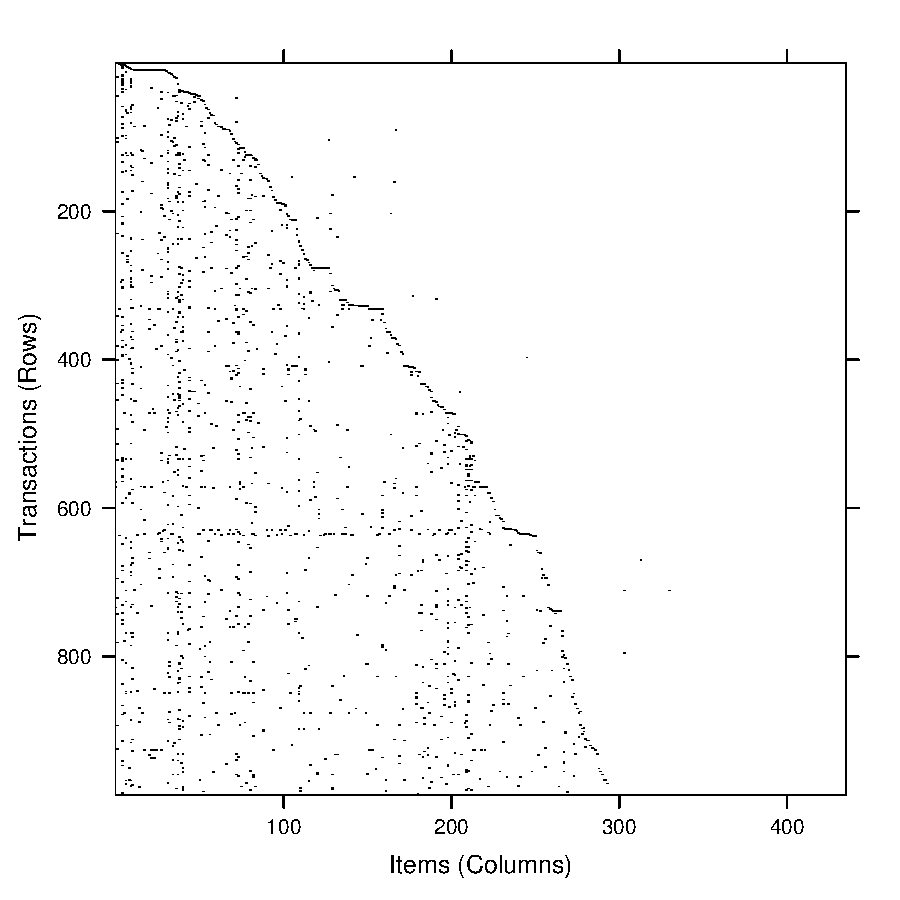
\includegraphics[width=10cm]{arules-epub}
\caption{The Epub data set (year 2003).}
\label{fig:imageEpub}
\end{figure}

The plot is a direct visualization of the binary incidence matrix where
the the dark dots represent the ones in the matrix.  From the plot we
see that the items in the data set are not evenly distributed.  In fact,
the white area to the top right side suggests, that in the beginning of
2003 only very few items were available (less than 50) and then during
the year more items were added until it reached a number of around 300
items. Also, we can see that there are some transactions in the data set
which contain a very high number of items (denser horizontal lines).
These transactions need further investigation since they could originate
from data collection problems (e.g., a web robot downloading many
documents from the publication site).  To find the very long
transactions we can use the \func{size} and select very long
transactions (containing more than 20 items).

\begin{Schunk}
\begin{Sinput}
> transactionInfo(Epub2003[size(Epub2003) > 20])
\end{Sinput}
\begin{Soutput}
    transactionID           TimeStamp
301  session_56e2 2003-04-29 05:30:38
580  session_6308 2003-08-17 10:16:12
896  session_72dc 2003-12-29 12:35:35
\end{Soutput}
\end{Schunk}

We found three long transactions and printed the corresponding
transaction information. Of course, size can be used in a similar
fashion to remove long or short transactions.

Transactions can be inspected using \func{inspect}. 
Since the long transactions identified above would result in
a very long printout, we will inspect 
the first 5 transactions in the subset for 2003.

\begin{Schunk}
\begin{Sinput}
> inspect(Epub2003[1:5])
\end{Sinput}
\begin{Soutput}
  items     transactionID           TimeStamp
1 {doc_154}  session_4795 2003-01-01 12:59:00
2 {doc_3d6}  session_4797 2003-01-01 23:46:01
3 {doc_16f}  session_479a 2003-01-02 02:50:38
4 {doc_f4,                                   
   doc_11d,                                  
   doc_1a7}  session_47b7 2003-01-02 10:55:50
5 {doc_83}   session_47bb 2003-01-02 13:27:44
\end{Soutput}
\end{Schunk}

Most transactions contain one item. Only transaction 4 contains three items. 
For further inspection transactions can be converted into a list with:

\begin{Schunk}
\begin{Sinput}
> as(Epub2003[1:5], "list")
\end{Sinput}
\begin{Soutput}
$session_4795
[1] "doc_154"

$session_4797
[1] "doc_3d6"

$session_479a
[1] "doc_16f"

$session_47b7
[1] "doc_f4"  "doc_11d" "doc_1a7"

$session_47bb
[1] "doc_83"
\end{Soutput}
\end{Schunk}

Finally, transaction data in horizontal layout can be converted to
transaction ID lists in vertical layout using coercion.

\begin{Schunk}
\begin{Sinput}
> EpubTidLists <- as(Epub, "tidLists")
> EpubTidLists
\end{Sinput}
\begin{Soutput}
tidLists in sparse format with
 465 items/itemsets (rows) and
 3975 transactions (columns)
\end{Soutput}
\end{Schunk}

For performance reasons the transaction ID list
is also stored in a sparse matrix. To get a list, coercion to \class{list}
can be used.

\begin{Schunk}
\begin{Sinput}
> as(EpubTidLists[1:3], "list")
\end{Sinput}
\begin{Soutput}
$doc_154
 [1] "session_4795" "session_6082" "session_60dd" "session_67db"
 [5] "session_769c" "session_7ee3" "session_bd9d" "session_c591"
 [9] "session_ce9f" "session_cf4b" "session_e019"

$doc_3d6
 [1] "session_4797"    "session_4893"    "session_48f4"   
 [4] "session_4ca3"    "session_wu4450a" "session_52c6"   
 [7] "session_5712"    "session_58e3"    "session_5984"   
[10] "session_5b20"    "session_5c20"    "session_5dc0"   
[13] "session_5eac"    "session_wu4a129" "session_6599"   
[16] "session_673d"    "session_683e"    "session_wu4d25a"
[19] "session_6f2f"    "session_708a"    "session_7a0c"   
[22] "session_7de5"    "session_89db"    "session_9227"   
[25] "session_9941"    "session_a4d7"    "session_a8c0"   
[28] "session_c3c4"    "session_c546"    "session_ca44"   
[31] "session_d328"    "session_d5b4"   

$doc_16f
[1] "session_479a" "session_56e2" "session_630c" "session_72dc"
[5] "session_8b3e" "session_91ab" "session_a202" "session_a7b9"
\end{Soutput}
\end{Schunk}

In this representation each item has an entry
which is a vector of all transactions it occurs in.
\class{tidLists} can be directly used as input for mining algorithms which 
use such a vertical database layout to mine associations.

In the next example, we will see how a data set is created and
rules are mined.

\subsection{Example 2: Preparing and mining a 
questionnaire data set\label{sec:example-adult}}

As a second example, we prepare and mine questionnaire data.  We use the
Adult data set from the UCI machine learning repository
\citep{arules:Blake+Merz:1998} provided by package~\pkg{arules}.  This
data set is similar to the marketing data set used by
\cite{arules:Hastie+Tibshirani+Friedman:2001} in their chapter about
association rule mining.  The data originates from the U.S. census
bureau database and contains 48842 instances with 14 attributes like
age, work class, education, etc.  In the original applications of the
data, the attributes were used to predict the income level of
individuals.  We added the attribute \code{income} with levels
\code{small} and \code{large}, representing an income of
$\le$~USD~50,000 and $>$~USD~50,000, respectively.  This data is
included in \pkg{arules} as the data set \code{AdultUCI}.


\begin{Schunk}
\begin{Sinput}
> data("AdultUCI")
> dim(AdultUCI)
\end{Sinput}
\begin{Soutput}
[1] 48842    15
\end{Soutput}
\begin{Sinput}
> AdultUCI[1:2, ]
\end{Sinput}
\begin{Soutput}
  age        workclass fnlwgt education education-num     marital-status
1  39        State-gov  77516 Bachelors            13      Never-married
2  50 Self-emp-not-inc  83311 Bachelors            13 Married-civ-spouse
       occupation  relationship  race  sex capital-gain capital-loss
1    Adm-clerical Not-in-family White Male         2174            0
2 Exec-managerial       Husband White Male            0            0
  hours-per-week native-country income
1             40  United-States  small
2             13  United-States  small
\end{Soutput}
\end{Schunk}


\code{AdultUCI} contains a mixture of categorical and metric attributes and
needs some preparations before it can be transformed into
transaction data suitable for association mining.
First, we remove the two attributes \code{fnlwgt} and
\code{education-num}. The first attribute is a weight calculated
by the creators of the data set from control data provided by
the Population Division of the U.S. census bureau. 
The second removed attribute is just a numeric representation of the
attribute \code{education} which is also part of the data set.

\begin{Schunk}
\begin{Sinput}
> AdultUCI[["fnlwgt"]] <- NULL
> AdultUCI[["education-num"]] <- NULL
\end{Sinput}
\end{Schunk}

Next, we need to map the four remaining metric attributes (\code{age},
\code{hours-per-week}, \code{capital-gain} and \code{capital-loss}) to ordinal
attributes by building suitable categories.
We divide the attributes \code{age} and \code{hours-per-week}
into suitable categories using knowledge about typical age groups 
and working hours. 
For the two capital related attributes,
we create a category called \code{None} 
for cases which have no gains/losses. 
Then we further divide the group with gains/losses
at their median into the two categories \code{Low} and \code{High}.


\begin{Schunk}
\begin{Sinput}
> AdultUCI[["age"]] <- ordered(cut(AdultUCI[["age"]], c(15, 
+     25, 45, 65, 100)), labels = c("Young", "Middle-aged", 
+     "Senior", "Old"))
> AdultUCI[["hours-per-week"]] <- ordered(cut(AdultUCI[["hours-per-week"]], 
+     c(0, 25, 40, 60, 168)), labels = c("Part-time", "Full-time", 
+     "Over-time", "Workaholic"))
> AdultUCI[["capital-gain"]] <- ordered(cut(AdultUCI[["capital-gain"]], 
+     c(-Inf, 0, median(AdultUCI[["capital-gain"]][AdultUCI[["capital-gain"]] > 
+         0]), Inf)), labels = c("None", "Low", "High"))
> AdultUCI[["capital-loss"]] <- ordered(cut(AdultUCI[["capital-loss"]], 
+     c(-Inf, 0, median(AdultUCI[["capital-loss"]][AdultUCI[["capital-loss"]] > 
+         0]), Inf)), labels = c("none", "low", "high"))
\end{Sinput}
\end{Schunk}

Now, the data can be automatically recoded as
a binary incidence matrix by coercing the data set to
\class{transactions}.

\begin{Schunk}
\begin{Sinput}
> Adult <- as(AdultUCI, "transactions")
> Adult
\end{Sinput}
\begin{Soutput}
transactions in sparse format with
 48842 transactions (rows) and
 115 items (columns)
\end{Soutput}
\end{Schunk}

The remaining 115 categorical attributes were
automatically recoded into 115
binary items. During encoding the item labels were generated in the
form of 
\texttt{<\emph{variable name}>=<\emph{category label}>}. 
Note that for cases with missing values all items corresponding to the 
attributes with the missing values were set to zero.

\begin{Schunk}
\begin{Sinput}
> summary(Adult)
\end{Sinput}
\begin{Soutput}
transactions as itemMatrix in sparse format with
 48842 rows (elements/itemsets/transactions) and
 115 columns (items)

most frequent items:
           capital-loss=none            capital-gain=None 
                       46560                        44807 
native-country=United-States                   race=White 
                       43832                        41762 
           workclass=Private                      (Other) 
                       33906                       401333 

element (itemset/transaction) length distribution:
sizes
    9    10    11    12    13 
   19   971  2067 15623 30162 

   Min. 1st Qu.  Median    Mean 3rd Qu.    Max. 
   9.00   12.00   13.00   12.53   13.00   13.00 

includes extended item information - examples:
           labels variables      levels
1       age=Young       age       Young
2 age=Middle-aged       age Middle-aged
3      age=Senior       age      Senior

includes extended transaction information - examples:
  transactionID
1             1
2             2
3             3
\end{Soutput}
\end{Schunk}

The summary of the transaction data set gives a rough overview showing
the most frequent items, the length distribution of the transactions and
the extended item information which shows which variable and which value
were used to create each binary item. In the first example we see that
the item with label \code{age=Middle-aged} was generated by variable
\code{age} and level \code{middle-aged}.  

To see which items are important in the data set we can use the
\func{itemFrequencyPlot}. To reduce the number of items, we only plot
the item frequency for items with a support greater than 10\% (using the parameter \code{support}).  For
better readability of the labels, we reduce the label size with the
parameter \code{cex.names}. The plot is shown in Figure~\ref{fig:itemFrequencyPlot}.

\begin{Schunk}
\begin{Sinput}
> itemFrequencyPlot(Adult, support = 0.1, cex.names = 0.8)
\end{Sinput}
\end{Schunk}
\begin{figure}
\centering
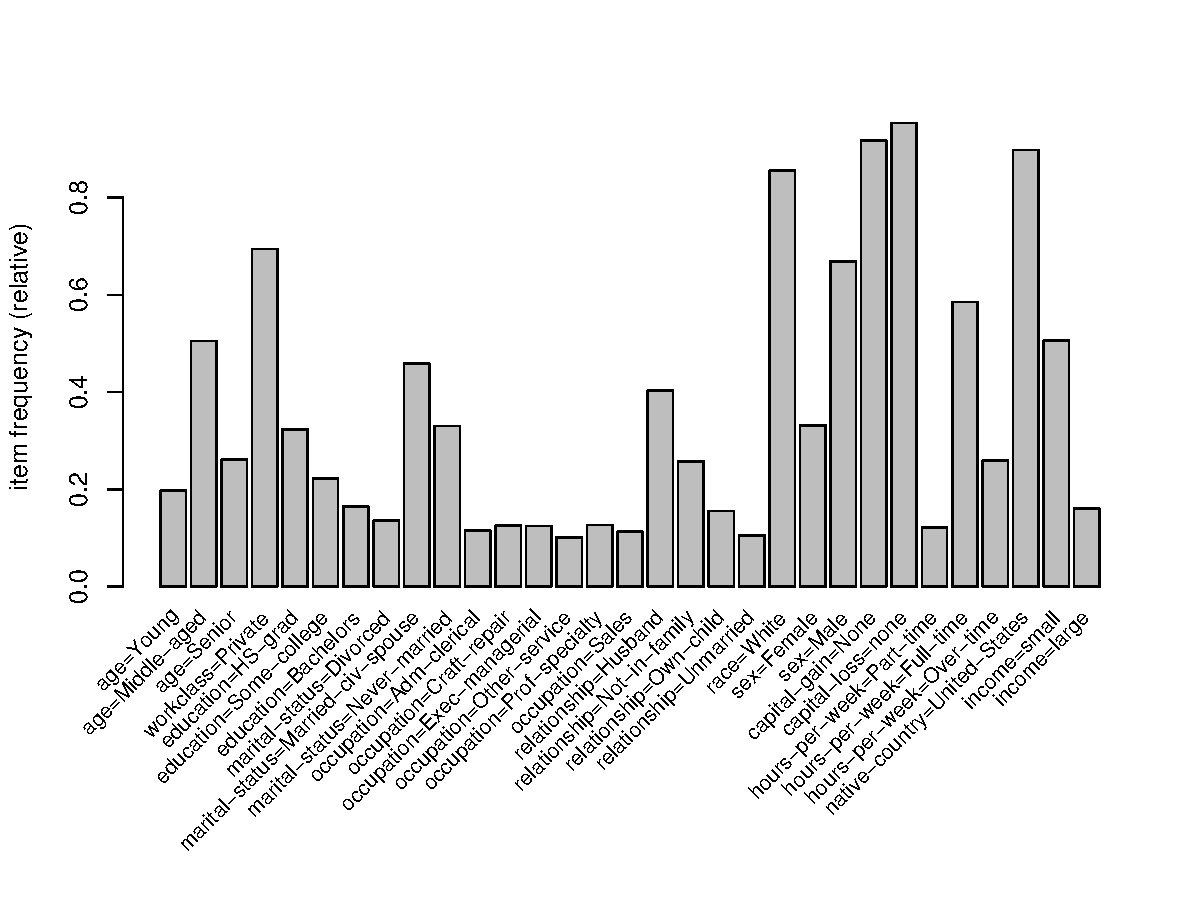
\includegraphics{arules-019}
\caption{Item frequencies of items in the Adult data set with support greater than 10\%.}
\label{fig:itemFrequencyPlot}
\end{figure}

Next, we call the function
\func{apriori} to find all rules (the default association type for
\func{apriori}) with a minimum support of 1\% and a confidence of 0.6.

\begin{Schunk}
\begin{Sinput}
> rules <- apriori(Adult, parameter = list(support = 0.01, 
+     confidence = 0.6))
\end{Sinput}
\begin{Soutput}
parameter specification:
 confidence minval smax arem  aval originalSupport support minlen maxlen
        0.6    0.1    1 none FALSE            TRUE    0.01      1      5
 target   ext
  rules FALSE

algorithmic control:
 filter tree heap memopt load sort verbose
    0.1 TRUE TRUE  FALSE TRUE    2    TRUE

apriori - find association rules with the apriori algorithm
version 4.21 (2004.05.09)        (c) 1996-2004   Christian Borgelt
set item appearances ...[0 item(s)] done [0.00s].
set transactions ...[115 item(s), 48842 transaction(s)] done [0.10s].
sorting and recoding items ... [67 item(s)] done [0.02s].
creating transaction tree ... done [0.09s].
checking subsets of size 1 2 3 4 5 done [0.99s].
writing ... [80215 rule(s)] done [0.03s].
creating S4 object  ... done [0.07s].
\end{Soutput}
\begin{Sinput}
> rules
\end{Sinput}
\begin{Soutput}
set of 80215 rules 
\end{Soutput}
\end{Schunk}

%The specified parameter values are validated and, for example,
%a support $> 1$ gives:
%
%<<error>>=
%error <- try(apriori(Adult, parameter = list(support = 1.3)))
%error
%@

First, the function prints the used parameters.  Apart from the
specified minimum support and minimum confidence, all parameters have
the default values. It is important to note that with parameter
\code{maxlen}, the maximum size of mined frequent itemsets, is by
default restricted to 5.  Longer association rules are only mined if
\code{maxlen} is set to a higher value.  After the parameter settings,
the output of the \proglang{C} implementation of the algorithm with timing
information is displayed.

The result of the mining algorithm is a set of 80215
rules.  For an overview of the mined rules \func{summary}
can be used.   It shows the number of rules, the most frequent items
contained in the left-hand-side and the right-hand-side and their
respective length distributions and summary statistics for the quality
measures returned by the mining algorithm.

\begin{Schunk}
\begin{Sinput}
> summary(rules)
\end{Sinput}
\begin{Soutput}
set of 80215 rules

rule length distribution (lhs + rhs):sizes
    1     2     3     4     5 
    6   432  4981 22127 52669 

   Min. 1st Qu.  Median    Mean 3rd Qu.    Max. 
  1.000   4.000   5.000   4.584   5.000   5.000 

summary of quality measures:
    support          confidence          lift        
 Min.   :0.01001   Min.   :0.6000   Min.   : 0.7201  
 1st Qu.:0.01364   1st Qu.:0.7542   1st Qu.: 1.0027  
 Median :0.02090   Median :0.8944   Median : 1.0433  
 Mean   :0.03770   Mean   :0.8501   Mean   : 1.2476  
 3rd Qu.:0.03966   3rd Qu.:0.9457   3rd Qu.: 1.2355  
 Max.   :0.95328   Max.   :1.0000   Max.   :20.6075  
\end{Soutput}
\end{Schunk}

As typical for association rule mining, the number of rules found is
huge.  To analyze these rules, for example, \func{subset} can be used to
produce separate subsets of rules for each item which resulted form the
variable \code{income} in the right-hand-side of the rule. At the same
time we require that the \code{lift} measure exceeds $1.2$.

\begin{Schunk}
\begin{Sinput}
> rulesIncomeSmall <- subset(rules, subset = rhs %in% "income=small" & 
+     lift > 1.2)
> rulesIncomeLarge <- subset(rules, subset = rhs %in% "income=large" & 
+     lift > 1.2)
\end{Sinput}
\end{Schunk}

We now have a set with rules for persons with a small income and a set
for persons with a large income.  For comparison, we inspect for both
sets the three rules with the highest confidence (using \func{SORT}).

%%{\samepage\small
\begin{Schunk}
\begin{Sinput}
> inspect(head(SORT(rulesIncomeSmall, by = "confidence"), n = 3))
\end{Sinput}
\begin{Soutput}
  lhs                               rhs               support confidence     lift
1 {workclass=Private,                                                            
   relationship=Own-child,                                                       
   sex=Male,                                                                     
   hours-per-week=Part-time}     => {income=small} 0.01154744  0.7058824 1.394689
2 {workclass=Private,                                                            
   marital-status=Never-married,                                                 
   sex=Male,                                                                     
   hours-per-week=Part-time}     => {income=small} 0.01517137  0.6951220 1.373428
3 {workclass=Private,                                                            
   occupation=Other-service,                                                     
   relationship=Own-child,                                                       
   capital-gain=None}            => {income=small} 0.01617460  0.6942004 1.371607
\end{Soutput}
\begin{Sinput}
> inspect(head(SORT(rulesIncomeLarge, by = "confidence"), n = 3))
\end{Sinput}
\begin{Soutput}
  lhs                                    rhs               support confidence     lift
1 {marital-status=Married-civ-spouse,                                                 
   capital-gain=High,                                                                 
   native-country=United-States}      => {income=large} 0.01562180  0.6849192 4.266398
2 {marital-status=Married-civ-spouse,                                                 
   capital-gain=High,                                                                 
   capital-loss=none,                                                                 
   native-country=United-States}      => {income=large} 0.01562180  0.6849192 4.266398
3 {relationship=Husband,                                                              
   race=White,                                                                        
   capital-gain=High,                                                                 
   native-country=United-States}      => {income=large} 0.01302158  0.6846071 4.264454
\end{Soutput}
\end{Schunk}
%%}

From the rules we see that workers in the private sector working part-time or
in the service industry tend to have a small income
while persons with high capital gain who are born in the US tend to have a
large income.
This example shows that using subset selection and sorting a
set of mined associations can be
analyzed even if it is huge.

Finally, the found rules can be written to disk to be shared 
with other applications. To save rules in plain text format 
the function \func{WRITE} is used. The 
following command saves a set of rules as the file named `data.csv' in 
comma separated value (CSV) format.

\begin{Schunk}
\begin{Sinput}
> WRITE(rulesIncomeSmall, file = "data.csv", sep = ",", col.names = NA)
\end{Sinput}
\end{Schunk}

Alternatively, with package~\pkg{pmml}~\cite{arules:Williams:2008} the rules
can be saved in PMML (Predictive Modelling Markup Language), a standardized
XML-based representation used my many data mining tools. Note that \pkg{pmml}
requires the package~\pkg{XML} which might not be available for all operating
systems. 

\begin{Schunk}
\begin{Sinput}
> library("pmml")
> rules_pmml <- pmml(rulesIncomeSmall)
> saveXML(rules_pmml, file = "data.xml")
\end{Sinput}
\end{Schunk}

The saved data can now be easily shared and used by other applications. 
Itemsets (with \func{WRITE} also transactions) can be 
written to a file in the same way.

\subsection{Example 3: Extending arules with a new interest measure\label{sec:example-allconf}}

In this example, we show how easy it is to add a new interest measure,
using \emph{all-confidence} as introduced by
\cite{arules:Omiecinski:2003}.  The all-confidence of an itemset~$X$ is
defined as

\begin{equation}
\mbox{all-confidence}(X) = \frac{\mathrm{supp}(X)}
{\mathrm{max}_{I \subset X} \mathrm{supp}(I)}
\label{equ:all_conf}
\end{equation}

This measure has the property $\mathrm{conf}(I \Rightarrow X \setminus
I) \ge \mbox{all-confidence}(X)$ for all $I \subset X$.  This means that
all possible rules generated from itemset~$X$ must at least have a
confidence given by the itemset's all-confidence value.
\cite{arules:Omiecinski:2003} shows that the support in the denominator
of equation~\ref{equ:all_conf} must stem from a single item and thus can
be simplified to $\max_{i \in X} \mathrm{supp}(\{i\})$.

To obtain an itemset to calculate all-confidence for, we mine frequent
itemsets from the previously used Adult data set using the Eclat
algorithm.

\begin{Schunk}
\begin{Sinput}
> data("Adult")
> fsets <- eclat(Adult, parameter = list(support = 0.05), control = list(verbose = FALSE))
\end{Sinput}
\end{Schunk}

For the denominator of all-confidence we need to find all mined single
items and their corresponding support values. In the following we 
create a named vector where the names are the column numbers of the 
items and the values are their support.

\begin{Schunk}
\begin{Sinput}
> singleItems <- fsets[size(items(fsets)) == 1]
> singleSupport <- quality(singleItems)$support
> names(singleSupport) <- unlist(LIST(items(singleItems), decode = FALSE))
> head(singleSupport, n = 5)
\end{Sinput}
\begin{Soutput}
       66        63       111        60         8 
0.9532779 0.9173867 0.8974243 0.8550428 0.6941976 
\end{Soutput}
\end{Schunk}

Next, we can calculate the all-confidence using
Equation~\ref{equ:all_conf} for all itemsets.  The single item support
needed for the denomination is looked up from the named vector
\code{singleSupport} and the resulting measure is added to the set's
quality data frame.

\begin{Schunk}
\begin{Sinput}
> itemsetList <- LIST(items(fsets), decode = FALSE)
> allConfidence <- quality(fsets)$support/sapply(itemsetList, 
+     function(x) max(singleSupport[as.character(x)]))
> quality(fsets) <- cbind(quality(fsets), allConfidence)
\end{Sinput}
\end{Schunk}

The new quality measure is now part of the set of itemsets.
\begin{Schunk}
\begin{Sinput}
> summary(fsets)
\end{Sinput}
\begin{Soutput}
set of 5908 itemsets

most frequent items:
           capital-loss=None native-country=United-States 
                        2301                         2245 
           capital-gain=None                   race=White 
                        2236                         2107 
           workclass=Private                      (Other) 
                        1784                        13555 

element (itemset/transaction) length distribution:sizes
   1    2    3    4    5 
  36  303 1078 2103 2388 

   Min. 1st Qu.  Median    Mean 3rd Qu.    Max. 
  1.000   4.000   4.000   4.101   5.000   5.000 

summary of quality measures:
    support        allConfidence    
 Min.   :0.05004   Min.   :0.05249  
 1st Qu.:0.06230   1st Qu.:0.06986  
 Median :0.08124   Median :0.09349  
 Mean   :0.11114   Mean   :0.13111  
 3rd Qu.:0.12554   3rd Qu.:0.14326  
 Max.   :0.95328   Max.   :1.00000  

includes transaction ID lists: FALSE 
\end{Soutput}
\end{Schunk}

It can be used to manipulate the set. For example, we can look at the
itemsets which contain an item related to education (using partial match with \code{\%pin\%}) and sort them by
all-confidence (we filter itemsets of length 1 first, since they have
per definition an all-confidence of~1).

\begin{Schunk}
\begin{Sinput}
> fsetsEducation <- subset(fsets, subset = items %pin% "education")
> inspect(SORT(fsetsEducation[size(fsetsEducation) > 1], by = "allConfidence")[1:3])
\end{Sinput}
\begin{Soutput}
  items                        support allConfidence
1 {education=HS-grad,                               
   hours-per-week=Full-time} 0.2090209     0.3572453
2 {education=HS-grad,                               
   income=small}             0.1807051     0.3570388
3 {workclass=Private,                               
   education=HS-grad}        0.2391794     0.3445408
\end{Soutput}
\end{Schunk}

The resulting itemsets show that the item high school graduate (but no
higher education) is highly associated with working full-time, a small
income and working in the private sector.  All-confidence is 
along with many other measures of interestingness already
implemented in \pkg{arules} as the function \func{interestMeasure}.

\subsection{Example 4: Sampling}
In this example, we show how sampling
can be used in \pkg{arules}. We use again the Adult data set.

\begin{Schunk}
\begin{Sinput}
> data("Adult")
> Adult
\end{Sinput}
\begin{Soutput}
transactions in sparse format with
 48842 transactions (rows) and
 115 items (columns)
\end{Soutput}
\end{Schunk}

To calculate a reasonable sample size $n$, we use the formula developed
by \cite{arules:Zaki+Parthasarathy+Li+Ogihara:1997} and presented in 
Section~\ref{sec:sample}. We choose a minimum support of 5\%.
As an acceptable error rate for support $\epsilon$ we choose 10\% and
as the confidence level ($1-c$) we choose 90\%. 

\begin{Schunk}
\begin{Sinput}
> supp <- 0.05
> epsilon <- 0.1
> c <- 0.1
> n <- -2 * log(c)/(supp * epsilon^2)
> n
\end{Sinput}
\begin{Soutput}
[1] 9210.34
\end{Soutput}
\end{Schunk}

The resulting sample size is considerably smaller than the size of the
original database.
With \func{sample} we produce a sample of size $n$ with replacement from
the database.


\begin{Schunk}
\begin{Sinput}
> AdultSample <- sample(Adult, n, replace = TRUE)
\end{Sinput}
\end{Schunk}

The sample can be compared with the 
database (the population) using an item frequency plot.
The item frequencies in the sample are displayed as bars and the
item frequencies in the original database are represented by 
the line. For better readability of the labels, we
only display frequent items in the plot and reduce
the label size with the parameter \code{cex.names}.
The plot is shown in Figure~\ref{fig:itemFrequencyPlot2}.

\begin{Schunk}
\begin{Sinput}
> itemFrequencyPlot(AdultSample, population = Adult, support = supp, 
+     cex.names = 0.7)
\end{Sinput}
\end{Schunk}
\begin{figure}
\centering
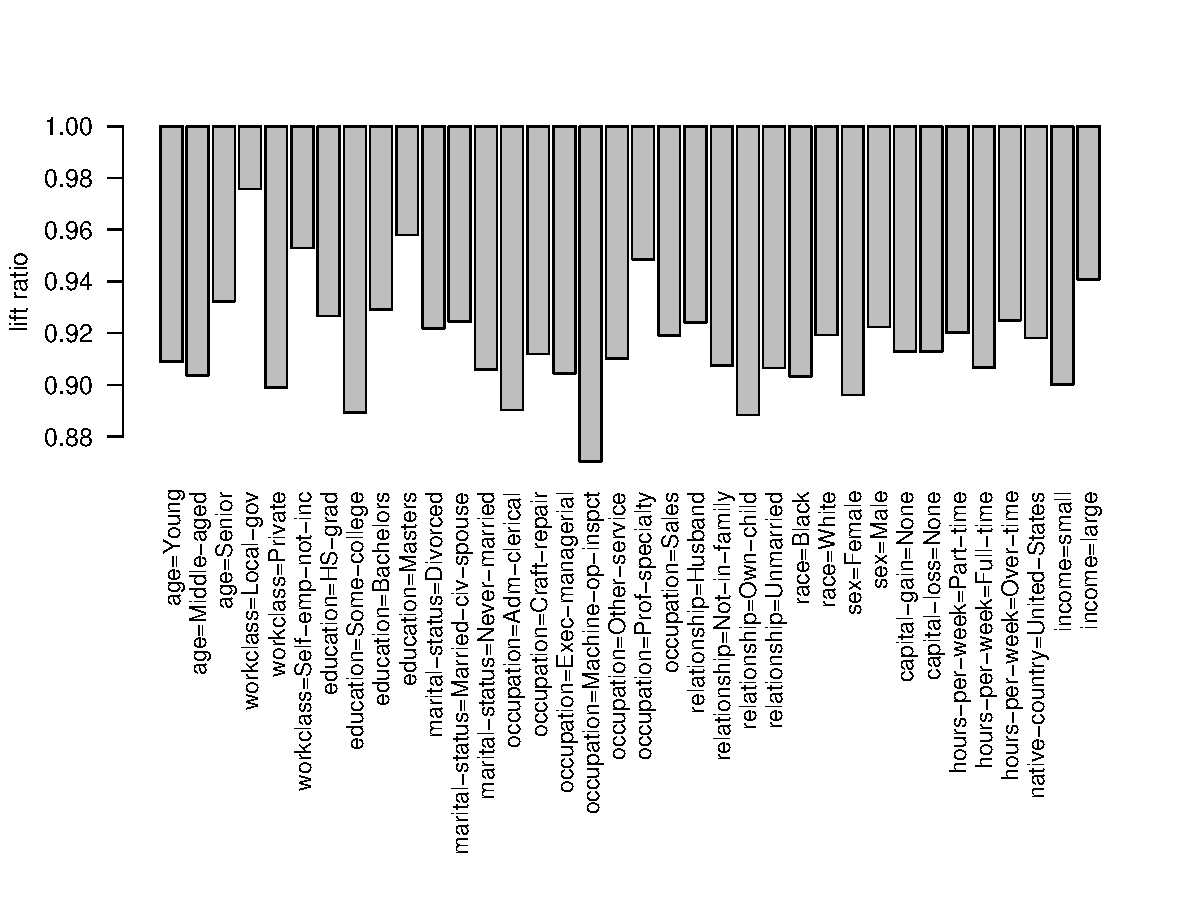
\includegraphics{arules-035}
\caption{Item frequencies in a sample of the Adult data set (bars) compared to 
the complete data set (line).}
\label{fig:itemFrequencyPlot2}
\end{figure}

Alternatively,
a sample can be compared with the population using the lift ratio 
(with \code{lift = TRUE}).
The lift ratio for each item $i$ is 
$P(i | \mathit{sample}) / P(i | \mathit{population})$ where the 
probabilities are estimated by the item frequencies.
A lift ratio of one indicates that the items occur in the sample
in the same proportion as in the population. A lift ratio greater than one 
indicates that the item is over-represented in the sample and vice versa.
With this plot, 
large relative deviations for less frequent items can be identified
visually
(see Figure~\ref{fig:itemFrequencyPlot3}). 

\begin{Schunk}
\begin{Sinput}
> itemFrequencyPlot(AdultSample, population = Adult, support = supp, 
+     lift = TRUE, cex.names = 0.9)
\end{Sinput}
\end{Schunk}
\begin{figure}
\centering
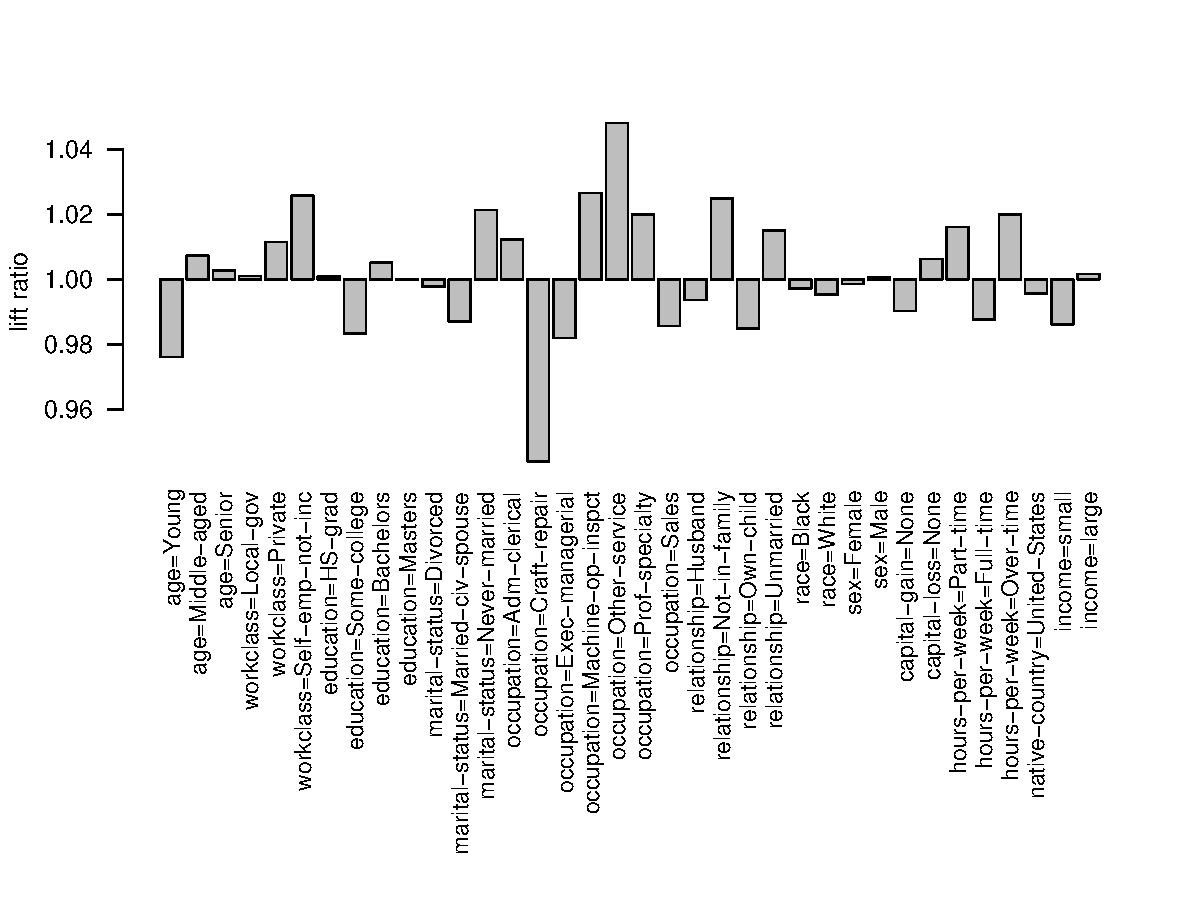
\includegraphics{arules-037}
\caption{Deviations of the item frequencies in the sample from 
the complete Adult data set.}
\label{fig:itemFrequencyPlot3}
\end{figure}

To compare the speed-up reached by sampling we use the Eclat algorithm
to mine frequent itemsets on both, the database and the sample
and compare the system time (in seconds) used for mining.

\begin{Schunk}
\begin{Sinput}
> time <- system.time(itemsets <- eclat(Adult, parameter = list(support = supp), 
+     control = list(verbose = FALSE)))
> time
\end{Sinput}
\begin{Soutput}
   user  system elapsed 
  0.552   0.000   0.550 
\end{Soutput}
\begin{Sinput}
> timeSample <- system.time(itemsetsSample <- eclat(AdultSample, 
+     parameter = list(support = supp), control = list(verbose = FALSE)))
> timeSample
\end{Sinput}
\begin{Soutput}
   user  system elapsed 
  0.120   0.000   0.119 
\end{Soutput}
\end{Schunk}

The first element of the vector returned by \func{system.time}
gives the (user) CPU time 
needed for the execution of the statement in its argument.
Therefore,
mining the sample instead of the whole data base results in a speed-up
factor of:
\begin{Schunk}
\begin{Sinput}
> time[1]/timeSample[1]
\end{Sinput}
\begin{Soutput}
user.self 
      4.6 
\end{Soutput}
\end{Schunk}



To evaluate the accuracy for the itemsets mined from the sample, we
analyze the difference between the two sets.

\begin{Schunk}
\begin{Sinput}
> itemsets
\end{Sinput}
\begin{Soutput}
set of 5908 itemsets 
\end{Soutput}
\begin{Sinput}
> itemsetsSample
\end{Sinput}
\begin{Soutput}
set of 5902 itemsets 
\end{Soutput}
\end{Schunk}

The two sets have roughly the same size. To check if the sets contain
similar itemsets, we match the sets and see what fraction of
frequent itemsets found in the database were also found in the sample. 


\begin{Schunk}
\begin{Sinput}
> match <- match(itemsets, itemsetsSample, nomatch = 0)
> sum(match > 0)/length(itemsets)
\end{Sinput}
\begin{Soutput}
[1] 0.975457
\end{Soutput}
\end{Schunk}

Almost all frequent itemsets were found using the sample.
The summaries of the support of the frequent itemsets 
which were not found in the sample and the itemsets
which were frequent in the sample although they
were infrequent in the database give:

\begin{Schunk}
\begin{Sinput}
> summary(quality(itemsets[which(!match)])$support)
\end{Sinput}
\begin{Soutput}
   Min. 1st Qu.  Median    Mean 3rd Qu.    Max. 
0.05004 0.05047 0.05125 0.05161 0.05217 0.05639 
\end{Soutput}
\begin{Sinput}
> summary(quality(itemsetsSample[-match])$support)
\end{Sinput}
\begin{Soutput}
   Min. 1st Qu.  Median    Mean 3rd Qu.    Max. 
0.05005 0.05060 0.05114 0.05142 0.05201 0.05505 
\end{Soutput}
\end{Schunk}

This shows that only itemsets with support very close to the minimum support
were falsely missed or found.

For the frequent itemsets which were found in the database and in the
sample, we can calculate accuracy from the the error rate.

\begin{Schunk}
\begin{Sinput}
> supportItemsets <- quality(itemsets[which(match > 0)])$support
> supportSample <- quality(itemsetsSample[match])$support
> accuracy <- 1 - abs(supportSample - supportItemsets)/supportItemsets
> summary(accuracy)
\end{Sinput}
\begin{Soutput}
   Min. 1st Qu.  Median    Mean 3rd Qu.    Max. 
 0.8668  0.9593  0.9766  0.9712  0.9887  1.0000 
\end{Soutput}
\end{Schunk}

The summary shows that sampling resulted in finding the support of itemsets
with high accuracy. This small example illustrates 
that for extremely large databases or for application where mining time 
is important, sampling can be a powerful technique.


%% ------------------------------------------------------------------
%% ------------------------------------------------------------------

\section{Summary and outlook\label{sec:conclusion}}

With package \pkg{arules} we
provide the basic infrastructure which enables us to 
mine associations and analyze and manipulate the results. 
%easily combine
%association mining with clustering and visualization techniques already
%available in \proglang{R}.  
Previously, in \proglang{R} there was no such infrastructure available.
The main features of \pkg{arules} are:

\begin{itemize}
 \item Efficient implementation using sparse matrices.
 \item Simple and intuitive interface to manipulate and analyze
  transaction data, sets of itemsets and rules with subset selection and
  sorting.
 \item Interface to two fast mining algorithms.
 \item Flexibility in terms of adding new quality measures, and
  additional item and transaction descriptions which can be used for
  selecting transactions and analyzing resulting associations.
 \item Extensible data structure to allow for easy implementation of new
  types of associations and interfacing new algorithms.
\end{itemize}

There are several interesting possibilities to extend \pkg{arules}.  For
example, it would be very useful to interface algorithms which use
statistical measures to find ``interesting'' itemsets (which are not
necessarily frequent itemsets as used in an association rule context).
Such algorithms include implementations of the $\chi^2$-test based
algorithm by \cite{arules:Silverstein+Brin+Motwani:1998} or the baseline
frequency approach by \cite{arules:DuMouchel+Pregibon2001}.

Another interesting extension would be to interface synthetic data 
generators for fast evaluation and comparison of different mining algorithms.
The best known generator for
transaction data for mining association rules
was developed by~\cite{arules:Agrawal+Srikant:1994}.
Alternatively data can be generated by simple probabilistic models 
as done by
\cite{arules:Hahsler+Hornik+Reutterer:2005}.

%Finally, similarity measures between itemsets and rules can be
%implemented for \pkg{arules}. With such measures distance based
Finally, the impelentation of distance based
clustering could be used for visualization of associations 
\citep[see e.g.,][]{arules:Strehl+Gosh:2003}.

\section*{Acknowledgments}
Part of \pkg{arules} was developed  during the project 
``Statistical Computing with R'' funded by  of the
``Jubil\"aumsstiftung der WU Wien.''
The authors of \pkg{arules} would like to thank Christian Borgelt for the
implementation of Apriori and Eclat.


\bibliographystyle{abbrvnat}
\bibliography{arules,misc}

\end{document}

%%% Local Variables:
%%% mode: latex
%%% TeX-master: t
%%% End:
